\chapter{Multi-Armed Bandit Algorithms}

\begin{equation}
\label{eq:pearsoncorrelation} \tag{23}
sim(u, j)
 = \frac{\sum_{i \in I}\left(r_{u,i} - \overline{r_{u}} \right ) \times \left ( r_{j,i} - \overline{r_{j}} \right)}{\sqrt{\sum_{i \in I}\left(U_{u, i} - \overline{r}_{u}\right)^{2}}\times\sqrt{\sum\left(r_{j,i}-\overline{r_{j}}\right)^{2}}}
\end{equation}


\begin{figure}[h]
   {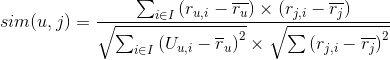
\includegraphics[width=2in]{img/PearsonEqn.gif}}
\end{figure}

The multi-armed bandit problem describes how a gambler is standing in front of multiple slot machines (one-armed bandits), needing to make decisions regarding which arm to pull with the intention of maximising the profit.
In the sense of recommender systems, this can be modelled as an actor or algorithm having multiple models to choose from, whereas the algorithm needs to decide which model to choose in order to give the best recommendation or make the best prediction.

\eqref{eq:pearsoncorrelation}


Background

The Multi-Armed Bandit problem is a decision-making problem for deciding on a model
to use when making predictions about the future[7]. It originates from the Markov decision process and was first formulated in 1952[8], however its concepts have documented
discussions from earlier and it at this point in time was not spoken of as Multi-Armed
Bandits. Since then there have been numerous different algorithms for how to solve it
with good performance.
Some of the bandit models’ practical use-areas have, for instance, consisted in providing
predictions regarding which projects that are most likely to be successful within different
research areas. This helps when determining how investments should be made to maximise the profit. It can also provide useful information regarding failing projects, so as
to stop the flow of money in an early stage. Other practical applications for the bandit
model have been clinical trials and adaptive routing, where it was used for optimisation.

3.2

The Algorithm

A general idea of The Multi-Armed Bandit problem is as follows:
14

3.2. THE ALGORITHM

CHAPTER 3. THE MAB ALGORITHM

1. Each arm is to be modelled as a lever, which upon being pulled, provides a reward
r belongs to -- R independently, from its own distribution in a setting where all arms have
their own distributions.
2. Mean values µ1 , µ2 , . . . , µn can then be computed, where n is the cardinality of the
set of distributions for all arms.
3. An agent plays on one lever at a time iteratively and observes the associated
rewards for each arm, respectively.
4. The objective of the agent is to maximise her winnings, the sum of the collected
rewards.
Within decision theory and probabilistic modelling, regret bounds are often used for
measuring negative emotion experience. That is when learning how a different course
of action would have resulted in a more favourable outcome. It is thereby desirable to
implement algorithms with as low regret bound as possible.
By modelling the Multi-Armed Bandit problem as a one-state Markov decision chain,
the total regret roh--- after m rounds can be seen as the expected difference between the sum
of total rewards from an optimal solution and the sum of the actual collected rewards
m
X

rbi

(3.1)

i=1

where rbi is the reward of the ith iteration.
Algorithm 1: Multi-armed bandit algorithm
Data: A: the arms, P: the purchases
1 previousP urchases  {}
2 forall the p in P do
3
a  policyLogic(A, previousP urchases) // Choose an arm depending on
policy
4
ListOfItems pullArm(a)
5
if p contains ListOfItems then
6
reward 1
7
else
8
reward 0
9
end
10
updateArm(a, reward) // Update the arm depending on success or failure
11
append(previousP urchases, p) // Append purchase p to the previous
12 end
policyLogic returns an arm a based on the policy logic described in section 3.3. pullArm
returns a list of items that a wants to recommend. updateArm is then updating a depending on whether the recommendations were successful or not. A recommendation is
15

3.3. POLICIES

CHAPTER 3. THE MAB ALGORITHM

considered successful if a recommended item is purchased by the specific user at a later
point in time. The update function is implemented differently for different implementations of the algorithm but the most common way is having alpha and beta variables that
get updated with success or failure. These parameters are then taken into consideration
when policyLogic is executed.

3.3

Policies

The main problem, using Multi-Armed Bandit algorithms, is to maintain a good ratio
between exploration versus exploitation, something that has been proved necessary to
consider in order to get as high cumulative profit as possible.

3.3.1
-greedy

The greedy[47] policy works by having a fixed value, that determines how much the
algorithm should explore and/or exploit. The policy starts with generating a random
number x. If the randomly generated value x is below it chooses an arm at random,
else it takes the arm with the best performance so far.
Algorithm 2: Multi-armed bandit algorithm with the -greedy policy
Data: A: the arms, P: the purchases, βa : tries of arm a, αa : successful tries of
arm a
1 Initialise all αa and βa to 0
2 forall the p in P do
3
x ← random[0,1]
4
if x < then
5
a ← random(A)
6
else
7
a ← argmax( αβaa )
8
end
9
ListOfItems ← pullArm(a)
10
if p contains ListOfItems then
11
inc(αa )
12
else
13
inc(βa )
14
end
15 end

3.3.2

Upper Confidence Bound

Upper confidence bound does not, in contrary to the greedy policy, continuously explore
throughout the whole running time of the algorithm with a fixed probability. Instead it
has a discovery phase, where it tries each arm once. After the discovery phase is finished,

16
3. POLICIES

CHAPTER 3. THE MAB ALGORITHM

it generates the policy for choosing an arm as
µa + λσa

(3.2)

where µa is the estimated reward for arm a, and σa a confidence bound measuring the
accuracy of our estimate, mean µa . The λ is, just as when using the greedy policy, a
fixed parameter to balance exploration versus exploitation.
A very simple and easy implementation, UCB1[48], can be performed by setting µa = αβaa
q P
and λσa = 2·lnβa β where αa is the number of times a specific arm has succeeded in
predicting a future purchase of an item, and βa is the number of times the arm has tried
to predict items in total.
Algorithm 3: Multi-armed bandit algorithm with the UCB1 policy
Data: A: the arms, P: the purchases, βa : tries of arm a, αa : successful tries of
arm a
1 Initialise all αa and βa to 0
2 forall the p in P do
q
a ← argmax( αβaa +

3
4
5
6
7
8
9
10

P
2·ln β
)
βa

ListOfItems ← pullArm(a)
if p contains ListOfItems then
inc(αa )
else
inc(βa )
end
end

3.3.3

Thompson Sampling

A policy on which a lot of recent focus have been put is a policy known as Thompson
Sampling [25, 26, 49, 50, 51], which unlike the UCB1 policy goes back to the exploration
phase faster when a previously well performing arm starts failing. It is also different in
comparison with the so called greedy policy which constantly keeps on exploring by
some fixed factor. Using Thomson Sampling exploration is instead decaying over time,
as the algorithm finds one or more arms that outperforms the others. If, however, there
is a change in the market, and a previously good arm suddenly starts to fail more often,
the method of Thompson Sampling will once again take a more exploratory approach as

17

3.4. CONTEXTUAL MAB

CHAPTER 3. THE MAB ALGORITHM

explained above.
Algorithm 4: Multi-armed bandit algorithm with Thompson Sampling without
decay
Data: A: the arms, P: the purchases, βa : tries of arm a, αa : successful tries of
arm a, B: beta-distribution function, λ: decay-factor
1 Initialise all αa and βa to 1
2 λ = 1.0
3 forall the p in P do
4
forall the a in A do
5
sa ← B(αa , βa )
6
end
7
a ← arg max (sa )
8
ListOfItems ← pullArm(a)
9
βa ← βa · λ
10
αa ← αa · λ
11
if p contains ListOfItems then
12
inc(αa )
13
else
14
inc(βa )
15
end
16 end
The goal of the Multi-Armed Bandit algorithm is to determine on which model to rely,
that would work best for the system at a specific point in time. Having the algorithm
choose among different statistical models, depending on what seems to be best at this
now, takes care of the problem where a specific method or formula which seemed to
work great one month might fail horribly the month after. This because of the algorithm
always choosing the best out of all available models, depending on actual premises from
this specific point in time. To be able to achieve this setting, the system needs to be selfupdating, something that Thompson Sampling is by default. The α and β parameters in
the algorithm can easily be adjusted to decay over time, simply by setting a decay-factor
λ to less than 1.0. If the intention is to trust old results rather than new, λ can also be
set to values higher than 1.0.

3.4

The Contextual Multi-Armed Bandit

The Contextual Multi-Armed Bandit Algorithm is a slight modified version of the original problem [11, 15]. Considering the phased solution in 3.2, for the Contextual MultiArmed Bandit, another phase is added between step two and step three. In addition to
the normal setting of a Multi-Armed Bandit there is now additional information that
might influence the choice of an agent regarding which arm to pull. Before actually
deciding, the agent now sees an n-dimensional feature vector, from now on referred to
as context vector, for each arm. The agent then uses these context vectors together

18

3.4. CONTEXTUAL MAB

CHAPTER 3. THE MAB ALGORITHM

with the rewards of each arm respectively upon deciding on what arm to pull in the
current iteration. The agent’s goal is to, overtime, gather enough information about the
relation between context vectors and rewards, so as to being able to predict which arm is
gonna yield the biggest reward only through observing the features of the context vectors.
The users, items and arms all have unique context vectors. When an item is bought
by a user, the context vector is updated for both the user and the item. If the arm
that was assigned the task of recommending an item made a successful prediction, the
system will update its α, as described in 1, to remember that the current arm had a good context vector and should be used more often.

